\documentclass[a4paper]{article}
\usepackage[utf8]{inputenc}
\usepackage[danish]{babel}
\usepackage[T1]{fontenc}
\renewcommand{\danishhyphenmins}{22}
\renewcommand{\arraystretch}{1.3}
\usepackage{amsmath,amssymb,bm,mathtools,rotating}

\usepackage{float}
\usepackage{listings,color}

\usepackage[top=3cm,bottom=3cm,left=3cm,right=3cm]{geometry}

\lstset{
  inputencoding=utf8,
  columns=flexible,
  basicstyle=\tt,
  language=bash,
  tabsize=3,
  showspaces=false,
  showstringspaces=false,
  breaklines=false
}

\title{02324: Milestone 1}
\author{
  s113933 - Flemming Madsen
  \and
    s103799 - Martin Hartvig
}

\begin{document}

\tableofcontents

\vspace{5cm}

\section{Timeregnskab} % (fold)
\label{sec:Timeregnskab}
\begin{tabular}{l l | c c c c c | c}

  \emph{Studienr} & \emph{Navn}
  & \begin{sideways}Design\end{sideways} 
  & \begin{sideways}Implementation\end{sideways} 
  & \begin{sideways}Test\end{sideways} 
  & \begin{sideways}Dokumentation\end{sideways} 
  & \begin{sideways}Andet\end{sideways} 
  & \begin{sideways}Total\end{sideways} \\
  \hline
  s113933 & Flemming Madsen              & 2 & 5  & 0  & 4 & 2 & 13 \\
  s093018 & Christian Walldeskog Nielsen & 4 & 6  & 0  & 0 & 0 & 10 \\
  s103799 & Martin Roland Hartvig        & 0 & 16 & 12 & 0 & 0 & 28 \\
  s113618 & Tobias Brasch                & 2 & 10 & 0  & 0 & 0 & 12 \\
  s113610 & Lavdrim Elmazi               & 0 & 0  & 0  & 0 & 5 & 5 \\
  \hline
  -       & -                            & 8 & 37 & 12 & 4 & 7 & 68
  
\end{tabular}

% section Timeregnskab (end)

\clearpage

%\tableofcontents

%\clearpage

\section{Vejledning} % (fold)
\label{sec:Vejledning}

% section Vejledning (end)

\clearpage

\section{Poster} % (fold)
\label{sec:Poster}

Ingen poster

% section Poster (end)

\clearpage

\section{Milestone 1} % (fold)
\label{sec:Milestone 1}

\subsection{Kravspecifikation} % (fold)
\label{sub:Kravspecifikation}

Kravspecifikation er læst og forstået, og vi ikke har umiddelbart yderlige ting at tilføje eller specificere ved den. Dette kan selvfølgelig ændre sig senere når vi når længere med processen med at designe en fornuftig dialog med operatøren

% subsection Kravspecifikation (end)

\subsection{Databasemodel} % (fold)
\label{sub:Databasemodel}

Vores database er stort set oversat fra de givne Data Transfer Objekts udleveret i projektbeskrivelsen. Angivelse af primary- og foreign-keys er sket ud fra nærlæsning af use case beskrivelser i opgavestillingen.

Se nedenstående figur for en grafisk repræsenation

\begin{figure}[H]
  \centering
  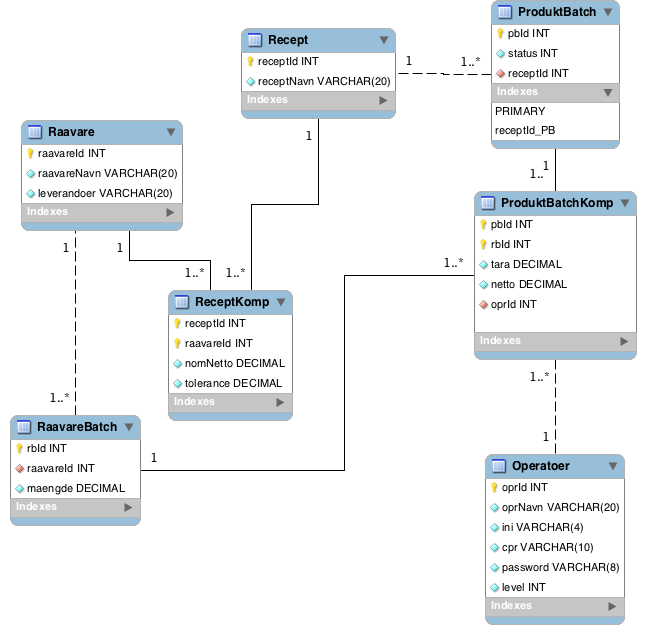
\includegraphics[scale=0.6]{graphics/db.png}
    \caption{Database}
\end{figure}

% subsection Databasemodel (end)

\subsection{Opgavens omfang og prioriteringer} % (fold)
\label{sub:Opgavens omfang og prioriteringer}

Vi satser på at nå alle de dele der er foreslået i opgavebeskrivelsen. Da vi i tidligere CDIO-delopgaver i fagene 02324 og 02325 har lavet størstedelen af de komponenter der skal bruges i det samlede system, anslår vi at have god tid til at få alle dele til at arbejde sammen, samt raffinere design/kode i de forskellige dele.

Det prioriteres også at have tid til at lave ordentlige tests af vores komponenter. På nuværende tidspunkt regner med at folk skriver tests til komponenter de ikke selv har lavet, dels for at sikre at man får en bedre viden om flere dele af koden, samt at testene såvidt muligt er objektive (altså ikke tester mod en specifik implementation, men mod specifik funktionalitet)

Hvis vi på et senere tidspunkt kommer i tidspres, vil vi priotere det højest at have et fuldt funktionelt system, som kan have mangler i brugerinterfacet. Vores vægtsimulator prioriteres kun til at understøtte de funktioner vi rent faktisk selv bruger i vores afvejnings styrings enhed.

% subsection Opgavens omfang og prioriteringer (end)

\subsection{Arbejdsfordeling} % (fold)
\label{sub:Arbejdsfordeling}

Vi har valgt at inddele den første del af opgaven i 4 komponenter og har uddelt det overordnede ansvar for dem som følger:

\begin{description}
  \item[Web service]\hfill
    \\Martin (UC 1-5)
  \item[Vægt simulator (GUI)]\hfill
    \\Tobias
  \item[MySQL DAO implementation]\hfill
    \\Christian
  \item[Afvejnings Styrings Enhed]\hfill
    \\Flemming (UC 6)
\end{description}

Lavdrim hjælper hvor der er behov, og folk hjælper løbende hinanden hvis behovet opstår.

% subsection Arbejdsfordeling (end)

\subsection{Tidsplan} % (fold)
\label{sub:Tidsplan}

Tidsplanen forventes løbende justeres

\paragraph{Uge 1} % (fold)
\label{par:Uge 1}

Vi satser på at vi sidst på dagen torsdag har de enkelte komponenter klar, således at sen torsdag/start fredag kan begynde at teste systemet som en sammensat helhed. Der opfordres til at folk løbende skriver på en rapport tekst der dokumenterer arbejds- og designprocessen for komponentet.

% paragraph Uge 1 (end)

\paragraph{Uge 2} % (fold)
\label{par:Uge 2}

Hvis systemet som helhed fungerer om fredagen, satser vi på at uge 2 bruges på at optimere samt udforme rapport og modeller. 

% paragraph Uge 2 (end)

% subsection Tidsplan (end)

% section Milestone 1 (end)


\end{document}


